\documentclass[border=2pt]{standalone}
\usepackage{tikz,amsmath}
\begin{document}
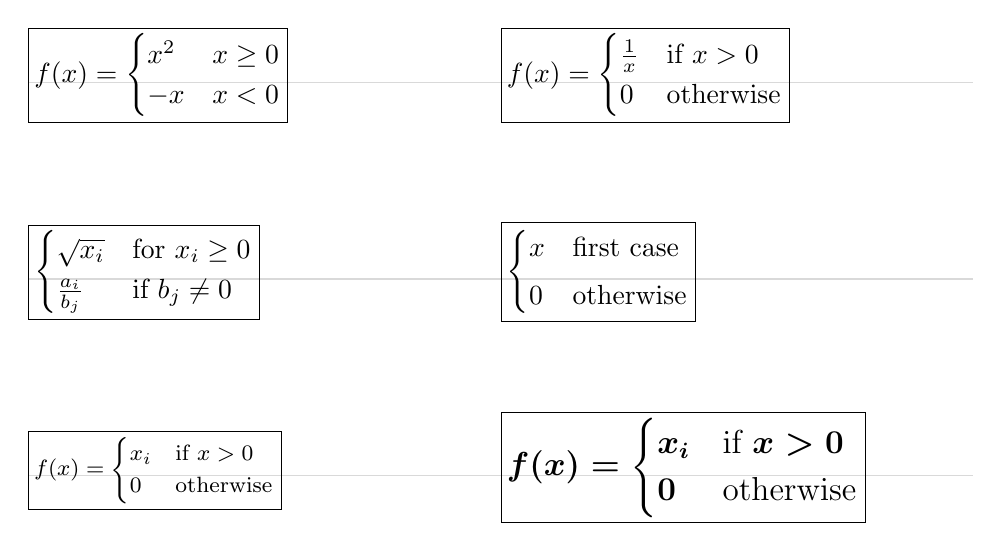
\begin{tikzpicture}
  \draw[gray!30] (0,0)--(12,0) (0,-2.5)--(12,-2.5) (0,-5)--(12,-5);
  \node[anchor=base west,draw,inner sep=2pt] at (0,0) {$f(x)=\begin{cases}x^2&x\geq0\\-x&x<0\end{cases}$};
  \node[anchor=base west,draw,inner sep=2pt] at (6,0) {$f(x)=\begin{cases}\frac{1}{x}&\text{if }x>0\\0&\text{otherwise}\end{cases}$};
  \node[anchor=base west,draw,inner sep=2pt] at (0,-2.5) {$\begin{cases}\sqrt{x_i}&\text{for }x_i\geq0\\\frac{a_i}{b_j}&\text{if }b_j\ne0\end{cases}$};
  \node[anchor=base west,draw,inner sep=2pt] at (6,-2.5) {$\begin{cases}x&\text{first case}\\[3pt]0&\text{otherwise}\end{cases}$};
  \node[anchor=base west,draw,inner sep=2pt,font=\footnotesize] at (0,-5) {$f(x)=\begin{cases}x_i&\text{if }x>0\\0&\text{otherwise}\end{cases}$};
  \node[anchor=base west,draw,inner sep=2pt,font=\large\boldmath] at (6,-5) {$f(x)=\begin{cases}x_i&\text{if }x>0\\0&\text{otherwise}\end{cases}$};
\end{tikzpicture}
\end{document}
